\section{Results}

\subsection{Estimating traits via PROSPECT inversion}

\begin{figure}
  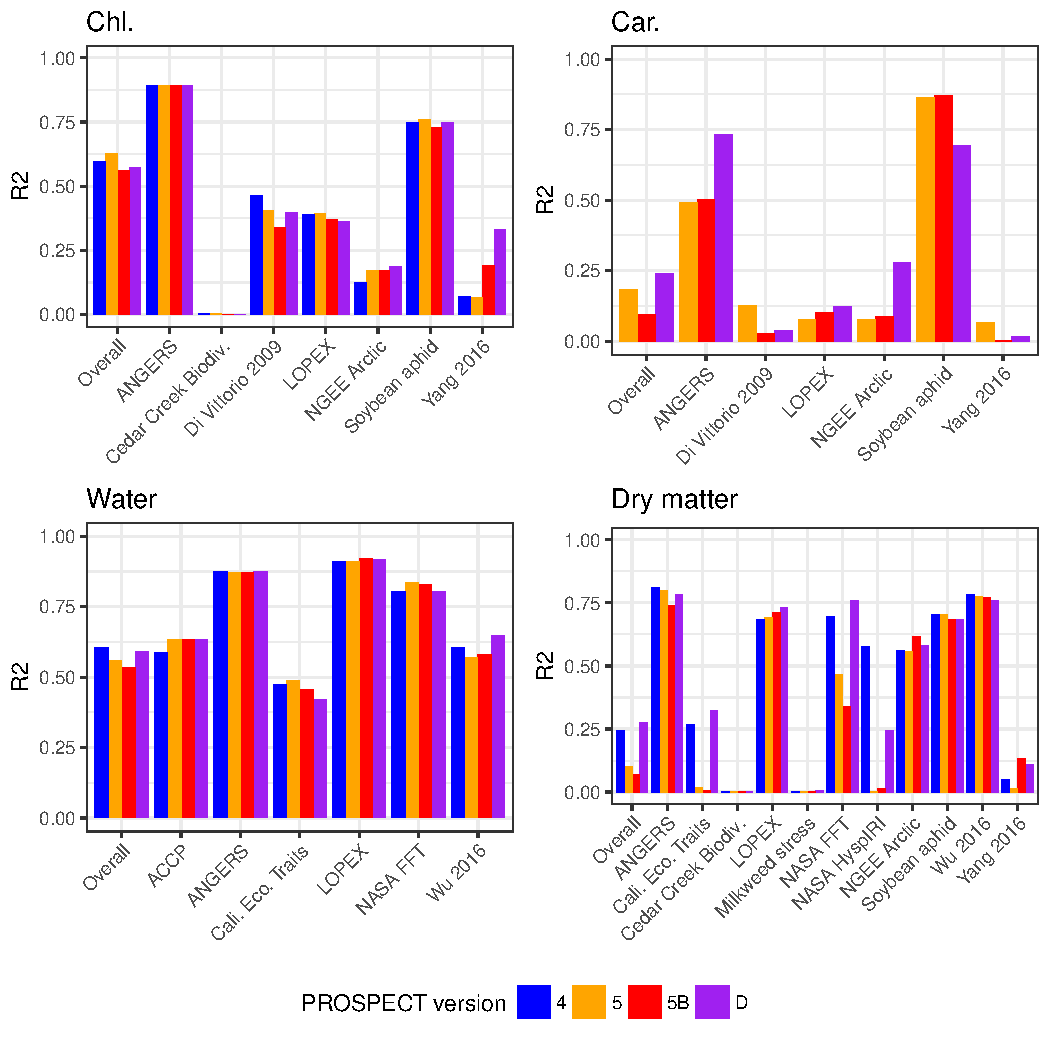
\includegraphics[width=\textwidth]{{figures/project_validation_summary}.pdf}
  \caption{\
    Validation of PROSPECT against observed trait values, by project and PROSPECT version
  }\label{fig:project_validation_summary}
\end{figure}

Across most projects and traits, the four different PROSPECT versions performed similarly in terms of their ability to retrieve traits (Figure~\ref{fig:project_validation_summary}).
For all versions of PROSPECT, leaf water content was consistently the most accurate trait retrieved, while retrievals of other traits were highly project-specific.
For several projects spanning a large range of species (Cali.\ Eco.\ Traits, NASA FFT, and NASA HyspIRI), moving from chlorophyll as the only pigment (PROSPECT 4) to chlorophyll and carotenoids (PROSPECT 5/5B) drastically reduced inversion accuracy of dry matter contents, but this accuracy was restored by the further addition of anthocyanins and modification of the refractive index in PROSPECT D (Figure~\ref{fig:project_validation_summary})
Inversion accuracy also varied significantly by project, which can largely be explained by differences in the species sampled across different projects (Supplementary Figures~\ref{fig:error_speciesbyproj_Cab}-\ref{fig:error_speciesbyproj_Cm}).
Because PROSPECT-D also retrieves anthocyanin content and generally performed as well or better than other versions, it was the version selected for subsequent analyses.
A more detailed validation for PROSPECT-D is shown in Figure~\ref{fig:prospect_D_validation}.

%TODO: More here?

\begin{figure}
  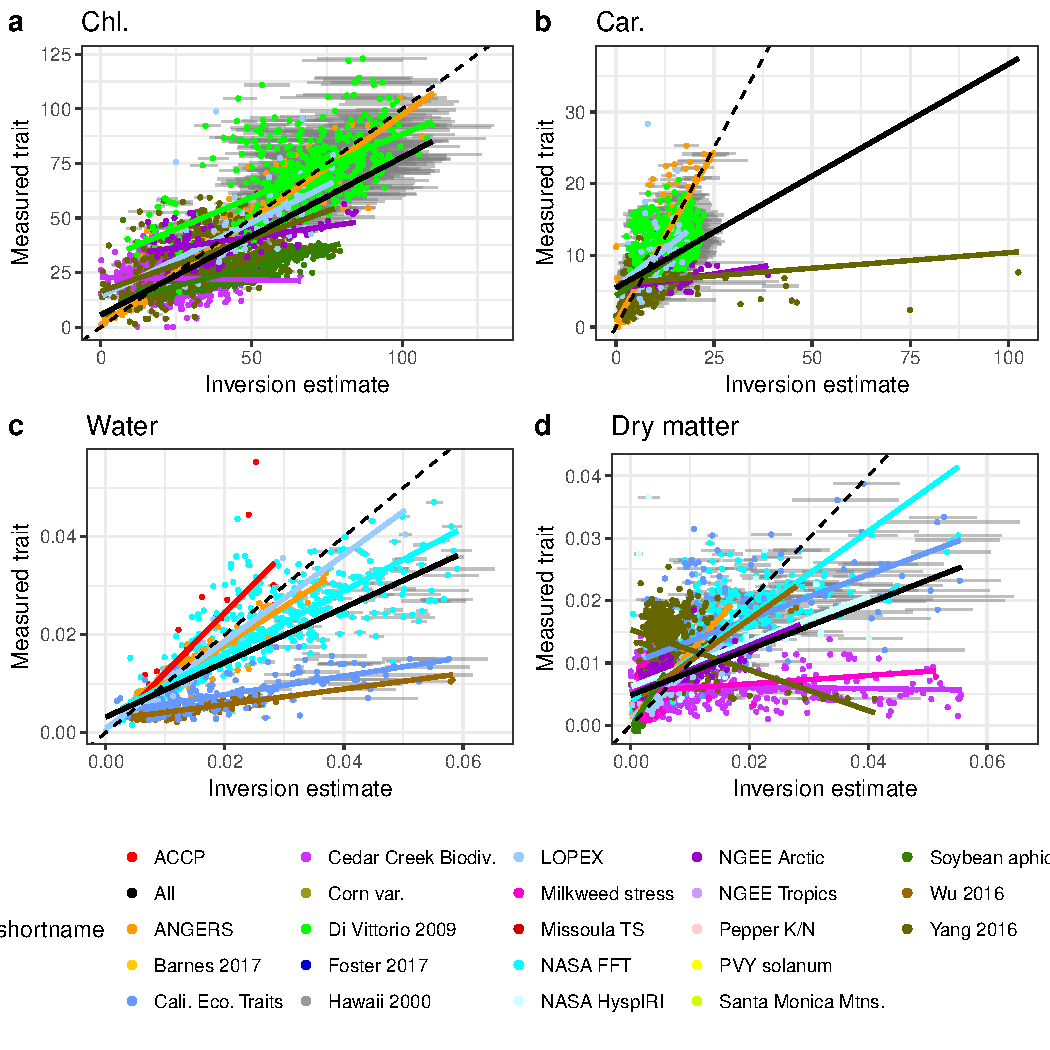
\includegraphics[width=\textwidth]{{figures/prospect_D_validation}.pdf}
  \caption{\
    Validation of PROSPECT-D against observed trait values.
    Grey lines indicate 95\% confidence intervals around trait estimates.
    Solid, colored lines are least-squares regressions fit to the data by project.
    The solid black line is a regression fit to all of the data all at once.
    The dashed black line is a 1 to 1 fit.
  }\label{fig:prospect_D_validation}
\end{figure}
% * <dietze@bu.edu> 2018-04-11T13:12:57.094Z:
% 
% Units are missing on the "measured trait"
% 
% ^.

\subsection{Drivers of variability in leaf optical traits}

\begin{figure}
  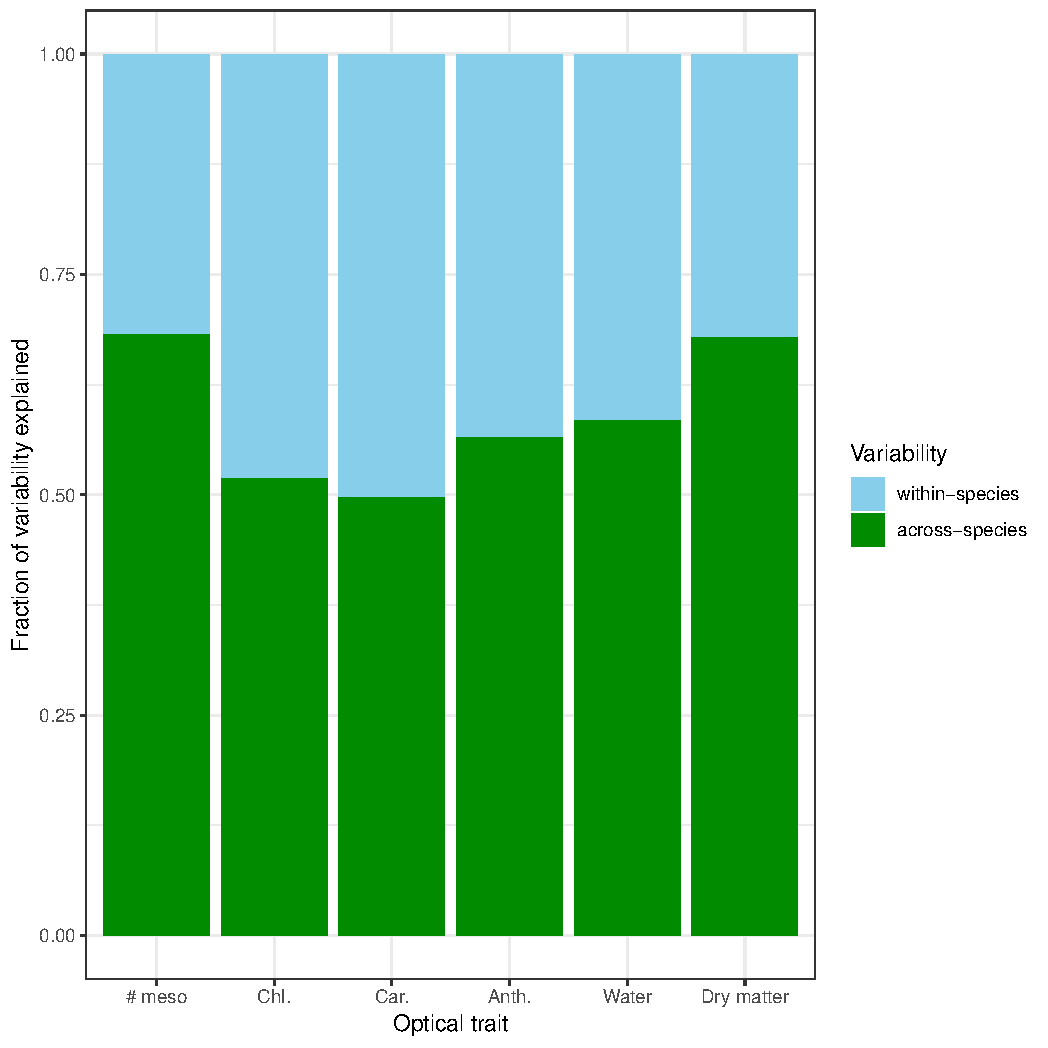
\includegraphics[width=\textwidth]{{figures/within_vs_across}.pdf}
  \caption{\
    Fraction of variance in each optical trait explained by species identity,
    based on analysis of variance on least-squares linear regression.
  }\label{fig:within_vs_across}
\end{figure}

\begin{figure}
  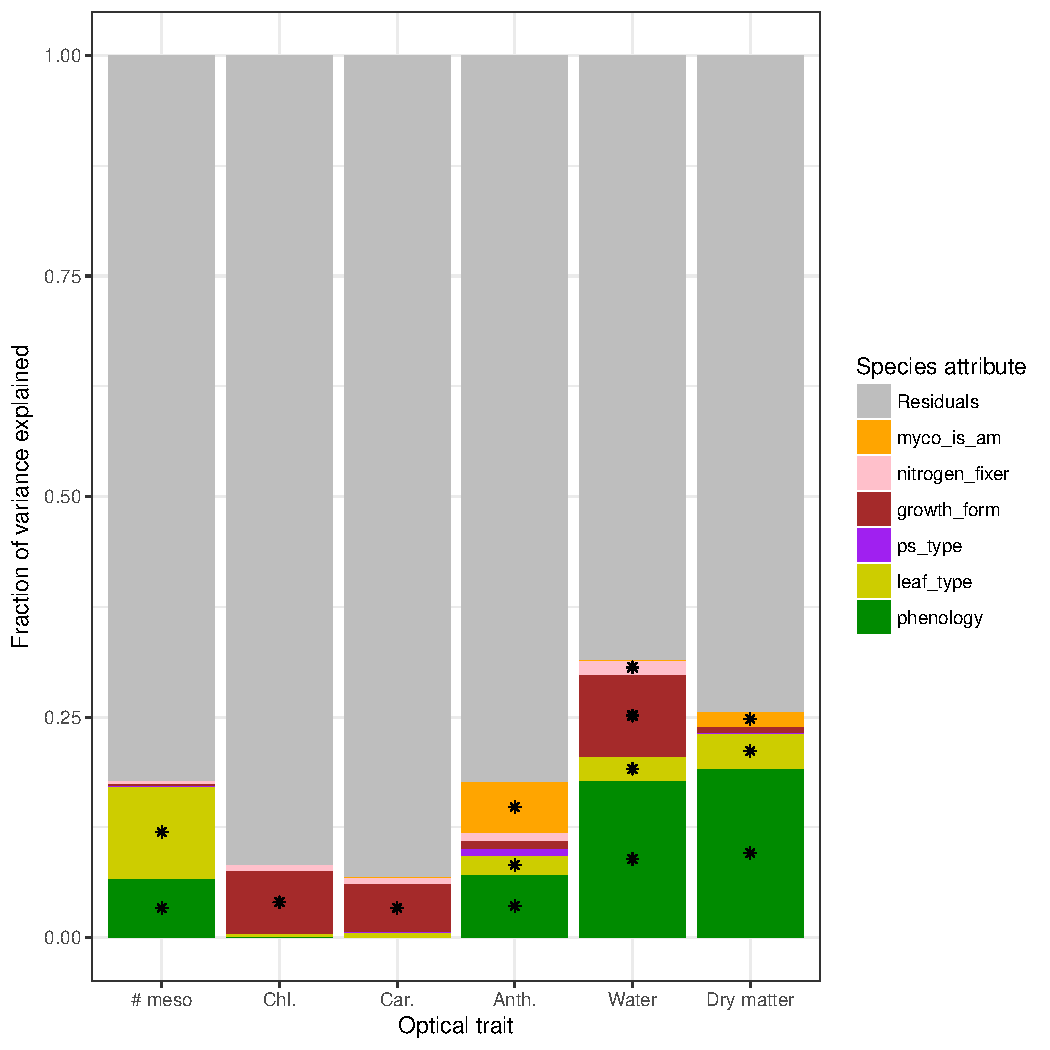
\includegraphics[width=\textwidth]{{figures/across_species_anova}.pdf}
  \caption{\
    Fraction of across-species variance in each optical trait (i.e.~species means) explained by species attributes,
    based on analysis of variance on least-squares linear regression.
    A star (*) indicates attribute effects significant at the 90\% confidence interval.
  }\label{fig:across_species_anova}
% * <fer.istem@gmail.com> 2018-04-11T19:46:59.552Z:
% 
% don't see ps_type defined anywhere
% 
% ^.
\end{figure}

Across all optical traits, roughly half of variability was explained by species identity (Figure~\ref{fig:within_vs_across}).
The variance across species means was largely ideosyncratic to species, with only up to 25\% of variance explainable by species attributes (Figure~\ref{fig:across_species_anova}).
The most important explanatory attribute was leaf phenology (deciduous vs.~evergreen), with occassional significant effects for leaf type (broad vs.~needle), growth form (woody vs.~herbaceous), and mycorrhizal association (arbuscular or non-arbuscular). 
% * <fer.istem@gmail.com> 2018-04-12T12:20:58.818Z:
% 
% how did you come up with this set of attributes?
% 
% what about tolerances (shade, drought), resistances (fire, herbivore) etc.
% 
% ^.
\begin{figure}
  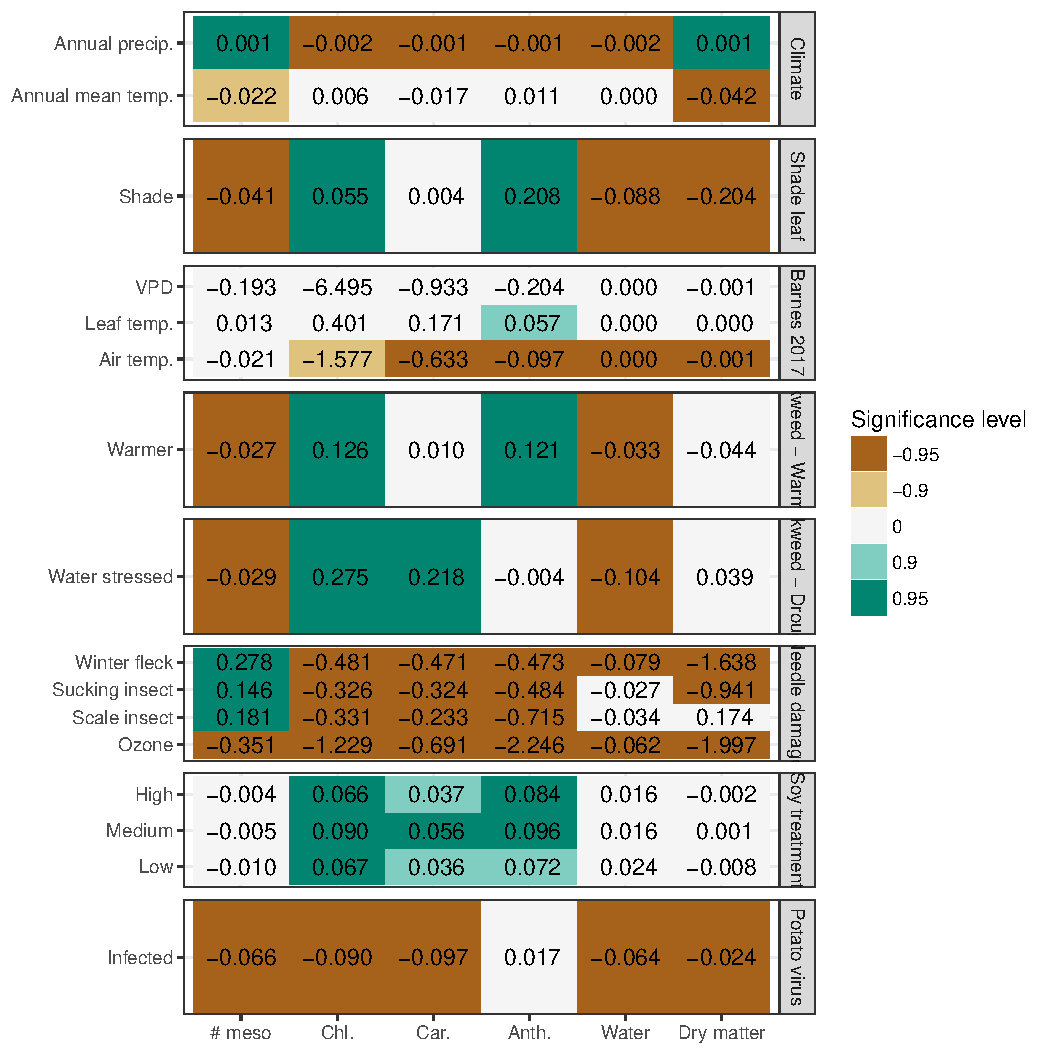
\includegraphics[width=\textwidth]{{figures/treatment_summary}.pdf}
  \caption{\
    Effects of different sources of intraspecific variability on traits estimated via PROSPECT inversion.
    Each value is the fixed effect slope on the corresponding trait normalized to zero mean and unit variance, as estimated from a linear fixed-effects model.
    Color brightness indicates degree of statistical significance (90 or 95\% confidence level), and color hues indicate effect direction (positive or negative).
  }\label{fig:treatment_summary}
\end{figure}

Leaf optical traits responded significantly to a range of natural and experimental stressors (Figure~\ref{fig:treatment_summary}).
Intraspecific variability in optical traits was weakly but, in some cases, significantly related to climate, with the strongest effects being declines in mesophyll structure and dry matter content with increasing temperature.
Based on leaf reflectance measurements of \textit{Populus deltoides} (eastern cottonwood) at the University of Arizona by Barnes et al.~(2017), \nocite{barnes_2017_beyond}
% * <dietze@bu.edu> 2018-04-11T13:20:03.945Z:
% 
% > Based on leaf reflectance
% Seems like a new paragraph. Switching from discussing overall correlations in the dataset to discussing results from specific experiments.
% 
% ^.
seasonal variations in leaf and air temperature had statistically significant but relatively small impacts on pigment concentrations.
Warming and drought experiments on \textit{Asclepias syriaca} (common milkweed) had strong and statistically significant effects on almost all optical traits, with both treatments leading to significant decreases in leaf water content and effective number of mesophyll layers and increases in pigments and dry matter content concentrations.
% * <dietze@bu.edu> 2018-04-11T13:21:29.452Z:
% 
% > Warming and drought experiments
% Are we moving on to different experiments at different site, or still Barnes? If the former, say where an provide citations.
% 
% ^.
In two independent studies, optical traits also responded significantly to chemical (ozone, winter fleck) and biotic (insects, viruses) stressors---all of these stressors significantly reduced concentrations of pigments, and typically also reduced water and dry matter contents, with ozone damage having the most significant effect.
% * <dietze@bu.edu> 2018-04-11T13:22:57.054Z:
% 
% > winter fleck
% What is winter fleck?
% 
% ^ <tmccabe@bu.edu> 2018-04-12T15:24:38.886Z:
% 
% +1
%
% ^.
% * <dietze@bu.edu> 2018-04-11T13:22:34.227Z:
% 
% > two independent studies
% CITATIONS!  Also, what systems/species where these studies in?
% 
% ^.
On the other hand, treatment of \textit{Glycine max} (soybean) with aphids resulted in a small but significant increase in pigment concentrations, with the strongest effect observed at medium-level treatment.
Finally, across the projects and species for which data were available for both sunlit and shaded leaves, shaded leaves had higher chlorophyll and anthocyanin concentrations and lower number of mesophyll layers and water and dry matter contents.
% * <dietze@bu.edu> 2018-04-11T13:24:20.646Z:
% 
% > across the projects and species for which data were available
% This should go up with the previous across study discussion points.
% 
% ^.

\begin{figure}
  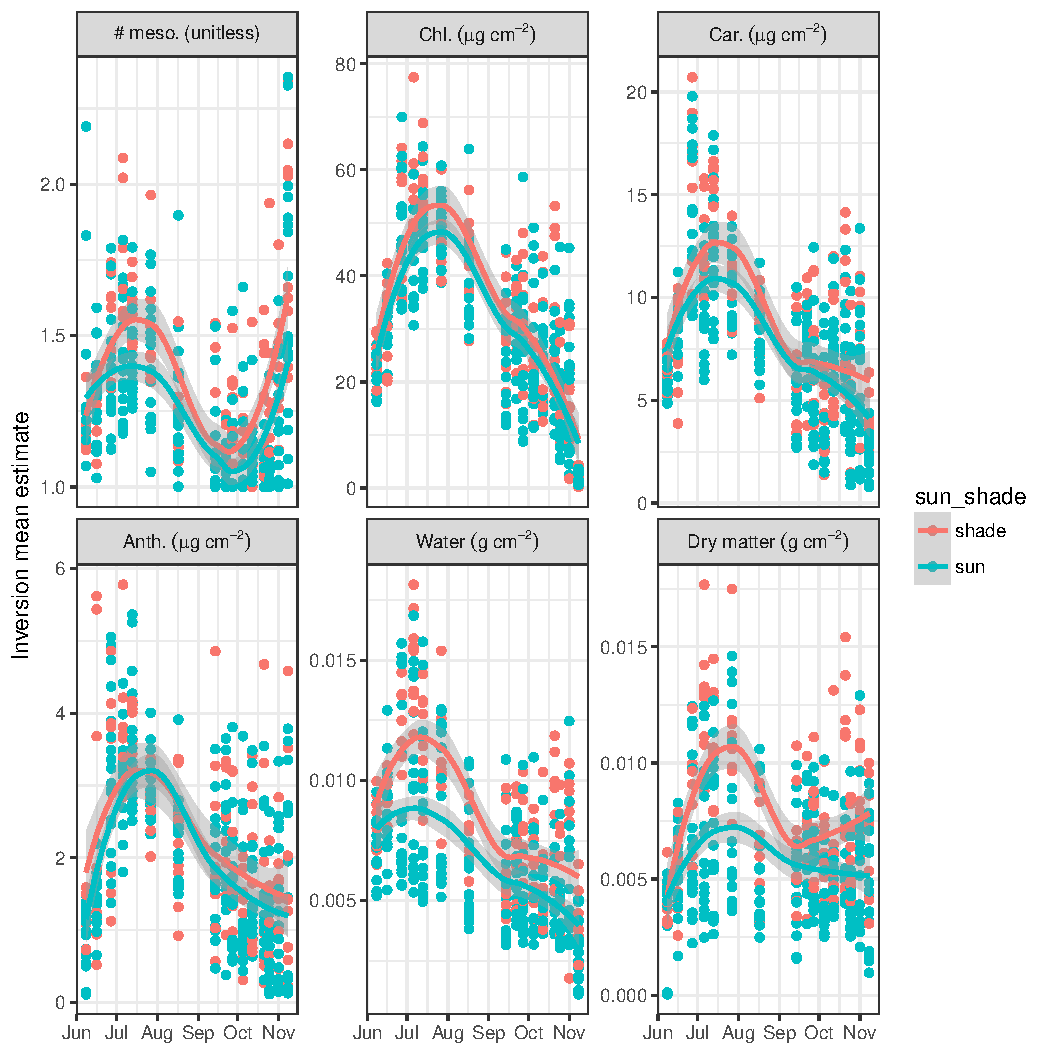
\includegraphics[width=\textwidth]{{figures/trait_phenology}.pdf}
  \caption{\
    Optical trait estimates through a season for Quercus rubra (red oak) at Martha's Vineyard, MA by Yang et al.~(2016).
    Colors indicate sunlit vs.~shaded leaves.
    Line is a LOESS best fit with shaded standard error.
  }\label{fig:trait_phenology}
  \nocite{yang_2016_seasonal}
\end{figure}

Where such measurements were available, leaf optical traits exhibited a strong phenological signal (Figure~\ref{fig:trait_phenology}).
All optical traits showed a peak in late July / early August, followed by a decline into the fall.
% * <dietze@bu.edu> 2018-04-11T13:26:03.488Z:
% 
% > All optical traits showed a peak in late July / early August, followed by a decline into the fall.
% 
% How could EVERYTHING within the leaf decline? Shouldn't something increase, if only on a relative basis?
% 
% ^.
However, the effective number of leaf mesophyll layers, and to a lesser extent, leaf dry matter content in sunlit leaves increased in the late fall. 
% * <dietze@bu.edu> 2018-04-11T13:26:48.623Z:
% 
% > effective number of leaf mesophyll layers, and to a lesser extent, leaf dry matter content in sunlit leaves increased in the late fall.
% 
% Make sure to come back to this in the discussion, as I'm not sure this is physiologically plausible.
% 
% ^.
With the exception of anthocyanin content, traits for sunlit leaves were higher and experienced a greater seasonal variability than shaded leaves.

\subsection{Trait correlations}

\begin{figure}
  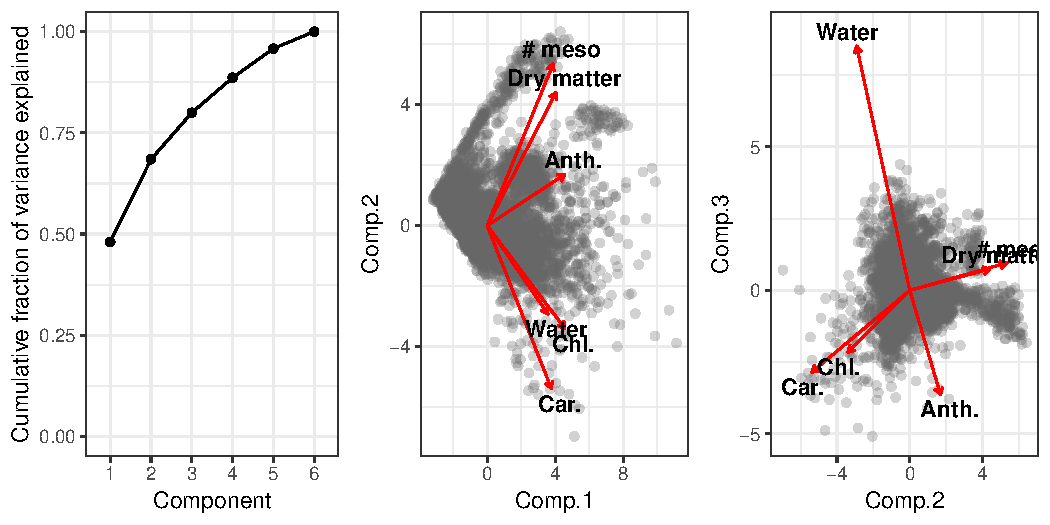
\includegraphics[width=\textwidth]{figures/prospect_pca.pdf}
  \caption{\
    Principal components analysis of optical trait correlation matrix. 
    (Left) Cumulative fraction of variance explained by each principal component.
    (Center, Right) Principal component scores and vectors for each optical trait for components 1 and 2 (center) and 2 and 3 (right).
  }\label{fig:prospect_pca}
\end{figure}

Optical traits estimated by PROSPECT are not mutually independent, but rather have some structure to their covariance (Figure~\ref{fig:prospect_pca}).
In the first two principal components, which collectively explain roughly 70\% of the variability, variation occurs along one of three axes---one defined by chlorophyll, carotenoid, and water contents, another defined by leaf structure and dry matter content, and a third defined by anthocyanin concentration.
% * <dietze@bu.edu> 2018-04-11T13:32:28.770Z:
% 
% > three axes
% Confusing -- how do the first two PCA have 3 axes?
% 
% ^ <emcowdery@gmail.com> 2018-04-12T06:37:57.092Z:
% 
% Three groupings that appear to fall along distinct axes?
% 
% ^.
% * <dietze@bu.edu> 2018-04-11T13:31:23.496Z:
% 
% > In the first two principal components
% 
% Looking back at the Methods, I can't find any mention of a plan to do a PCA. Never introduce new analyses in the Results.
% 
% ^.
Variation along the third principal component, which brings the cumulative variance up to roughly 80\%, is defined by a trade-off between water and anthocyanins.
% * <emcowdery@gmail.com> 2018-04-12T06:39:17.797Z:
% 
% > cumulative variance up to roughly 80\%
% But itself only adds ~10% 
% (It's just a wording thing, it's important to note that just the first 2 PCs add up to 80% but be clear about how little the second contributes in comparison the to the first) 
% 
% ^.

\begin{figure}
  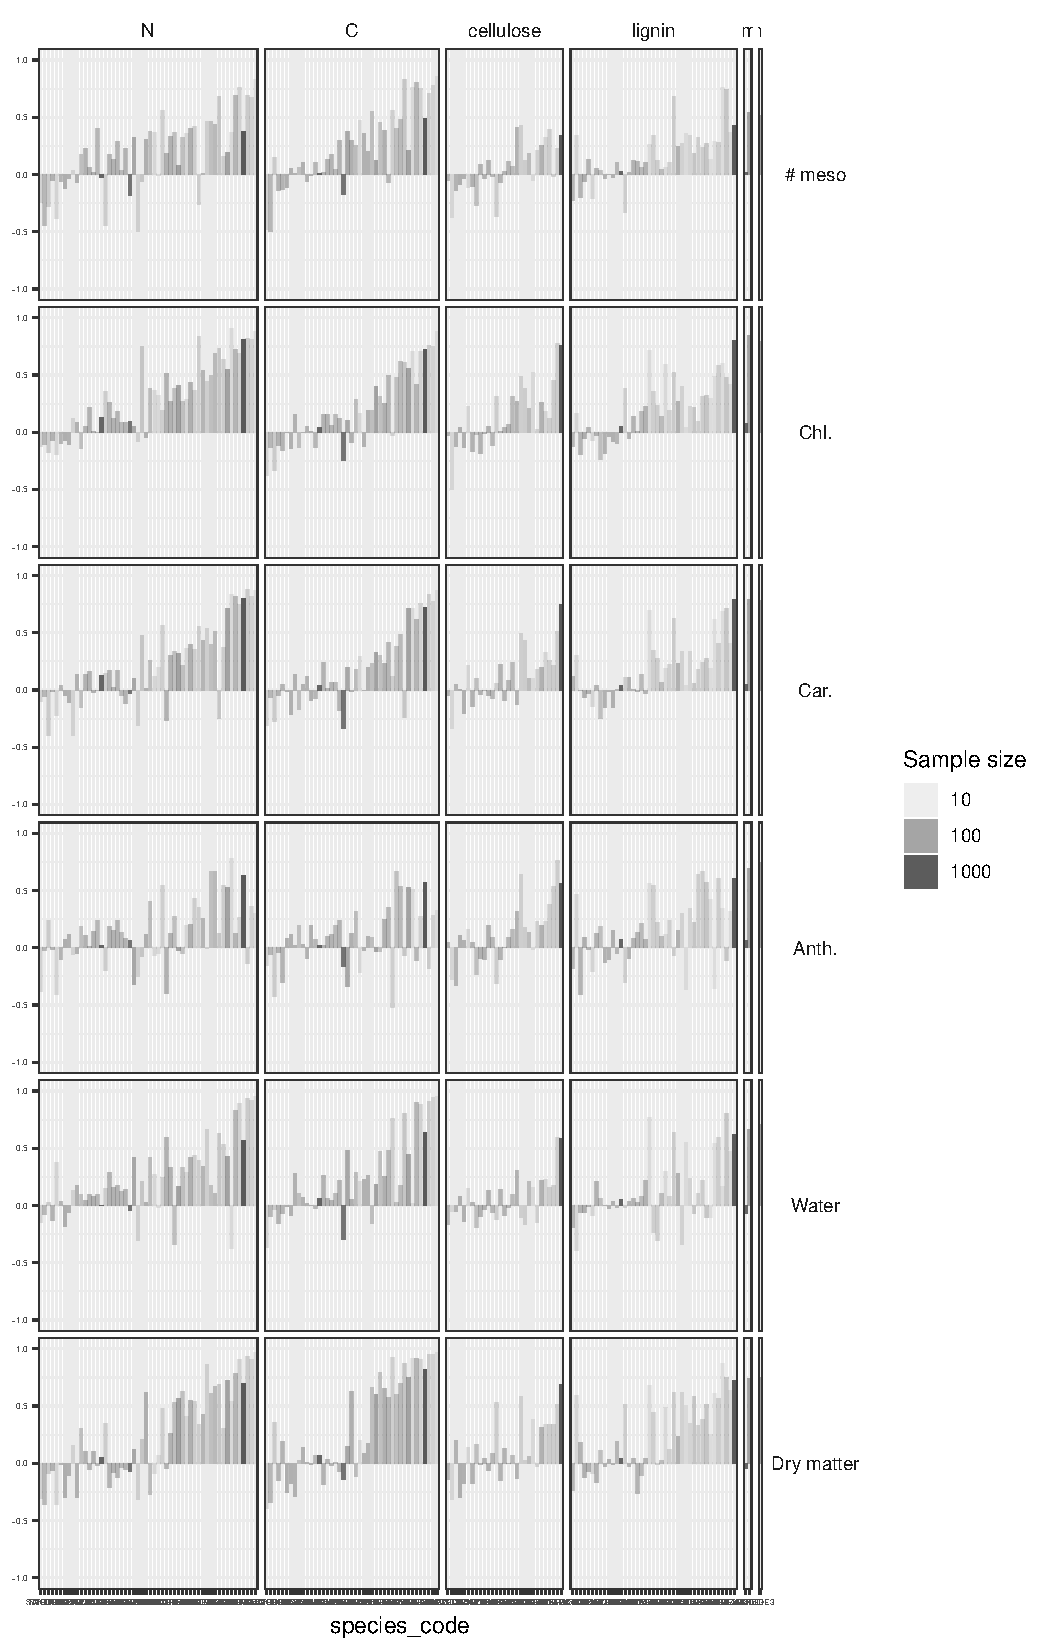
\includegraphics[width=\textwidth]{figures/trait_correlations_areabars.pdf}
  \caption{\
    Intra-specific pairwise correlations of optical traits with direct measurements of
    leaf N, C, cellulose, lignin, Vcmax, and Jmax.
    Darker colors indicate larger sample sizes.
    Species in each facet row are sorted by correlation averaged across all traits.
    Analysis was performed only for species with at least 10 pairwise observations of each trait.
% * <dietze@bu.edu> 2018-04-11T14:16:31.779Z:
% 
% Y-axis needs to be explained. Try to make this bigger so the font size isn't so small -- maybe put C and N on one page, and everything else on the next?
% 
% ^.
  }\label{fig:trait_correlations}
\end{figure}

Covariance of optical traits with six area-normalized traits---leaf nitrogen, carbon, cellulose, and lignin contents, Vcmax, and Jmax---was strongly species specific, but, in many cases, substantial (Figure~\ref{fig:trait_correlations}).
% * <dietze@bu.edu> 2018-04-11T14:13:48.873Z:
% 
% > strongly species specific
% 
% Did you not also look at the interspecific correlations? Everything below seems to be intraspecific.
% 
% ^.
In general, for any given species, most of the estimated optical traits exhibited similar correlations with the directly measured trait.
For instance, for soybean (GLMA4), all optical traits were positively correlated with leaf N, C, cellulose, and lignin, whereas for milkweed, all of these correlations were negligible.
Leaf nitrogen correlated best for the largest number of species with leaf chlorophyll and, to a slightly lesser extent, with dry matter content.
Leaf carbon and lignin were most consistently correlated with leaf dry matter content, while correlations with cellulose were more idiosyncratic.
Vcmax and Jmax were strongly positively correlated with all traits for \textit{Populus delotoides} (PODE3), but completely uncorrelated for milkweed (ASSY).

% TODO: Mass traits?

%On a mass basis, leaf number of mesophyll layers and dry matter contents were negatively correlated with direct pigment measurements and protein contents and weakly positively correlated with cellulose, hydrogen, fat, and non-structural carbohydrates.
%Pigments exhibited strong
